\documentclass[11pt,a4paper]{article}

% -----------------------------------------------------------------------------
% Essential Packages
% -----------------------------------------------------------------------------
\usepackage[utf8]{inputenc}
\usepackage[T1]{fontenc}
\usepackage{lmodern}
\usepackage[margin=0.9in]{geometry}
\usepackage{graphicx}
\usepackage{xcolor}
\usepackage{hyperref}
\usepackage{booktabs}
\usepackage{tabularx}
\usepackage{enumitem}
\usepackage{titlesec}
\usepackage{caption}
\usepackage{float}
\usepackage{fancyhdr}
\usepackage{microtype}

% -----------------------------------------------------------------------------
% Color Definitions (Nordic Palette Matching Project Architecture)
% -----------------------------------------------------------------------------
\definecolor{NordicTeal}{HTML}{0F766E}
\definecolor{NordicAmber}{HTML}{EA580C}
\definecolor{Charcoal}{HTML}{1C1917}
\definecolor{LightTeal}{HTML}{F0FDFA}
\definecolor{LightGray}{HTML}{F5F5F4}
\definecolor{MutedGray}{HTML}{78716C}
\definecolor{BorderGray}{HTML}{D6D3D1}

% -----------------------------------------------------------------------------
% Hyperlink Styling
% -----------------------------------------------------------------------------
\hypersetup{
    colorlinks=true,
    linkcolor=NordicTeal,
    citecolor=NordicTeal,
    urlcolor=NordicTeal,
    pdftitle={SE331 Continuous Assessment 1 (CA1) - Nadim},
    pdfauthor={Nadim}
}

% -----------------------------------------------------------------------------
% Section Heading Styling
% -----------------------------------------------------------------------------
\titleformat{\section}
  {\color{NordicTeal}\normalfont\Large\bfseries}
  {\thesection}{1em}{}[\color{NordicTeal}\titlerule]

\titleformat{\subsection}
  {\color{Charcoal}\normalfont\large\bfseries}
  {\thesubsection}{1em}{}

\titleformat{\subsubsection}
  {\color{Charcoal}\normalfont\normalsize\bfseries}
  {\thesubsubsection}{1em}{}

% -----------------------------------------------------------------------------
% Header and Footer
% -----------------------------------------------------------------------------
\pagestyle{fancy}
\fancyhf{}
\lhead{\footnotesize\textcolor{MutedGray}{SE331 -- Continuous Assessment 1 (CA1)}}
\rhead{\footnotesize\textcolor{MutedGray}{Nadim | Prototype \& UI/UX Design}}
\cfoot{\footnotesize\thepage}
\renewcommand{\headrulewidth}{0.4pt}

% -----------------------------------------------------------------------------
% Document Body
% -----------------------------------------------------------------------------
\begin{document}

% Title Block
\begin{center}
    {\scriptsize\textbf{\textcolor{NordicTeal}{\fbox{SE331 CONTINUOUS ASSESSMENT 1 (CA1) -- INDIVIDUAL TASK}}}}\\[0.8em]
    {\LARGE\textbf{\textcolor{Charcoal}{Prototype \& UI/UX Design Submission}}}\\[0.4em]
    {\large\textit{\textcolor{MutedGray}{Assigned Module: User Registration, Profile Management \& Onboarding Hub}}}\\[1.2em]
\end{center}

\vspace{-0.5em}

% -----------------------------------------------------------------------------
% 1. Student & Project Metadata
% -----------------------------------------------------------------------------
\section{Student \& Project Metadata}

\noindent
\begin{tabularx}{\textwidth}{@{} >{\bfseries\color{Charcoal}}p{3.2in} X @{}}
\toprule
Field & Details \\
\midrule
Student Name & Nadim \\
Student ID & \textcolor{NordicAmber}{\textbf{[Insert Your Student ID -- e.g., 211-35-XXXX]}} \\
Course Code \& Title & SE331 -- Software Engineering \\
Assessment Name & Continuous Assessment 1 (CA1): Prototype / UI/UX Design \\
Project Name & \textbf{JOB HUB} -- AI-Powered Smart Placement Platform \\
Assigned Git Branch & \url{https://github.com/Saif-AlSaad/JobHub/tree/Nadim} \\
Live Cloud Prototype & \url{https://saif-alsaad.github.io/JobHub/} \\
Local Prototype URL & \texttt{http://localhost:5173} \\
\bottomrule
\end{tabularx}

\vspace{1.5em}

% -----------------------------------------------------------------------------
% 2. Group Discussion & Page Division Summary
% -----------------------------------------------------------------------------
\section{Group Discussion \& Page Division Summary}

During the collaborative group phase, our team (\textit{Saif, Nadim, Rizvi}) listed all architectural screens required for the \textbf{JOB HUB} ecosystem. The screens and responsibilities were divided equally as follows:

\vspace{0.8em}
\noindent
\begin{tabularx}{\textwidth}{@{} l p{2.2in} X @{}}
\toprule
\textbf{Member} & \textbf{Assigned Module \& Screens} & \textbf{Core Design Responsibilities} \\
\midrule
\textbf{Nadim (Me)} & 
\textbf{User Onboarding \& Profile Hub}\newline
$\bullet$ User Registration Page (\texttt{/register})\newline
$\bullet$ Profile \& Resume Studio (\texttt{/profile})\newline
$\bullet$ Role Gateway \& Sign In (\texttt{/login}) & 
Dual-role sign up (Seeker/Recruiter), dynamic password strength entropy meter, interactive avatar modal, AI resume parser studio, interactive skill taxonomy, academic metrics, and geospatial placement radar. \\
\addlinespace
\textbf{Saif} & 
\textbf{Analytics \& Dashboards}\newline
$\bullet$ Candidate Dashboard (\texttt{/})\newline
$\bullet$ Recruiter Pipeline (\texttt{/recruiter})\newline
$\bullet$ Admin Governance (\texttt{/admin}) & 
Placement metrics scorecards, candidate Kanban pipelines, activity feeds, and platform administration. \\
\addlinespace
\textbf{Rizvi} & 
\textbf{Job Discovery \& Tracking}\newline
$\bullet$ Jobs Search \& Filters (\texttt{/jobs})\newline
$\bullet$ Job Details \& Match (\texttt{/jobs/:id})\newline
$\bullet$ Applications Tracker (\texttt{/applications}) & 
Job search filtering, match score breakdown card, application timeline tracking, and applicant review. \\
\bottomrule
\end{tabularx}

\vspace{1.5em}

% -----------------------------------------------------------------------------
% 3. Detailed Screen Architecture & Feature Breakdown
% -----------------------------------------------------------------------------
\section{Assigned Pages Architecture \& Feature Breakdown}

\subsection{Screen 1: User Registration Page (\texttt{/register})}
\begin{itemize}[leftmargin=1.5em, itemsep=0.3em]
    \item \textbf{Dual-Role Onboarding Switcher:} Allows immediate toggling between \textit{Job Seeker / Student} and \textit{Recruiter / Employer} directly inside the form. Automatically modifies labels and inputs (e.g., switches \textit{Full Name} to \textit{Company Name}).
    \item \textbf{Dynamic Password Entropy Meter:} Real-time password complexity evaluation across 4 discrete tiers (\textit{Weak, Fair, Good, Strong}) accompanied by an interactive color-coded progress indicator (Red $\rightarrow$ Amber $\rightarrow$ Teal $\rightarrow$ Emerald).
    \item \textbf{Form Security \& Validation:} Show/hide password toggles, confirm password equality check, and integrated Terms of Service consent.
    \item \textbf{Rapid Evaluation Helper:} Built-in \textit{"Fill sample info"} button enabling one-click test population for demonstrators.
\end{itemize}

\subsection{Screen 2: Candidate Profile \& Credentials Management (\texttt{/profile})}
\begin{itemize}[leftmargin=1.5em, itemsep=0.3em]
    \item \textbf{Interactive Avatar Management Studio:} Supports custom image upload with client-side HTML5 Canvas compression (sub-100 KB payload) and an interactive \textit{"Choose Sample Avatar"} modal with professional headshot presets.
    \item \textbf{AI Resume Parser Studio:} File upload zone for PDF/DOCX (up to 5 MB) with automated extraction of academic degree, CGPA, graduation data, and technical skills into the profile.
    \item \textbf{Dynamic Skills Taxonomy Manager:} Interactive skill chips with deletion ($\times$), custom skill entry with keyboard \texttt{Enter} support, and one-click suggested presets (\texttt{+ TypeScript}, \texttt{+ AWS}).
    \item \textbf{Academic Background \& CGPA Metrics:} Direct inputs for University/Institute, Degree/Major, Cumulative CGPA spinbutton, and professional headline.
    \item \textbf{Geospatial Placement Radar:} Campus/urban hub anchor selection (\textit{Savar Smart City, Banani}, etc.) and distance radius filter (\textit{2 km, 5 km, 10 km, 20 km}) with Haversine distance privacy protection.
    \item \textbf{Dual Recruiter Mode:} Authenticating as an employer seamlessly converts the profile into a corporate company management view (company size, industry, corporate website, Banani office anchor).
\end{itemize}

\vspace{1.5em}

% -----------------------------------------------------------------------------
% 4. UI/UX Design System Specification
% -----------------------------------------------------------------------------
\section{UI/UX Design System Specification}

\noindent
\begin{tabularx}{\textwidth}{@{} >{\bfseries\color{Charcoal}}p{1.8in} X @{}}
\toprule
Design Element & Specification \& Implementation \\
\midrule
Design Language & \textbf{Nordic Clean Minimalism \& Human-Centric Clarity} \\
Color Palette & Warm Canvas Paper (\texttt{\#FAF8F5}), Deep Charcoal Text (\texttt{\#1C1917}), Muted Slate (\texttt{\#57534E} / \texttt{\#E7E5E4}), Primary Candidate Teal (\texttt{\#0F766E}), Primary Recruiter Amber (\texttt{\#EA580C}), Success Emerald (\texttt{\#059669}). \\
Typography & Modern Sans-Serif hierarchy: H1 (24--26px bold), H2 (18--20px semibold), Body (13--14px regular), Microcopy (11--12px medium). \\
Micro-Interactions & Active button scale compression (\texttt{active:scale-95}), smooth CSS transitions (\texttt{200ms}), focus ring outlines for accessibility. \\
Accessibility (a11y) & Full compliance with WCAG 2.1 AA color contrast and keyboard navigation focus states. \\
\bottomrule
\end{tabularx}

\newpage

% -----------------------------------------------------------------------------
% 5. Visual Prototype Gallery & Screen Evidence
% -----------------------------------------------------------------------------
\section{Visual Prototype Gallery \& Screen Evidence}

\begin{figure}[H]
    \centering
    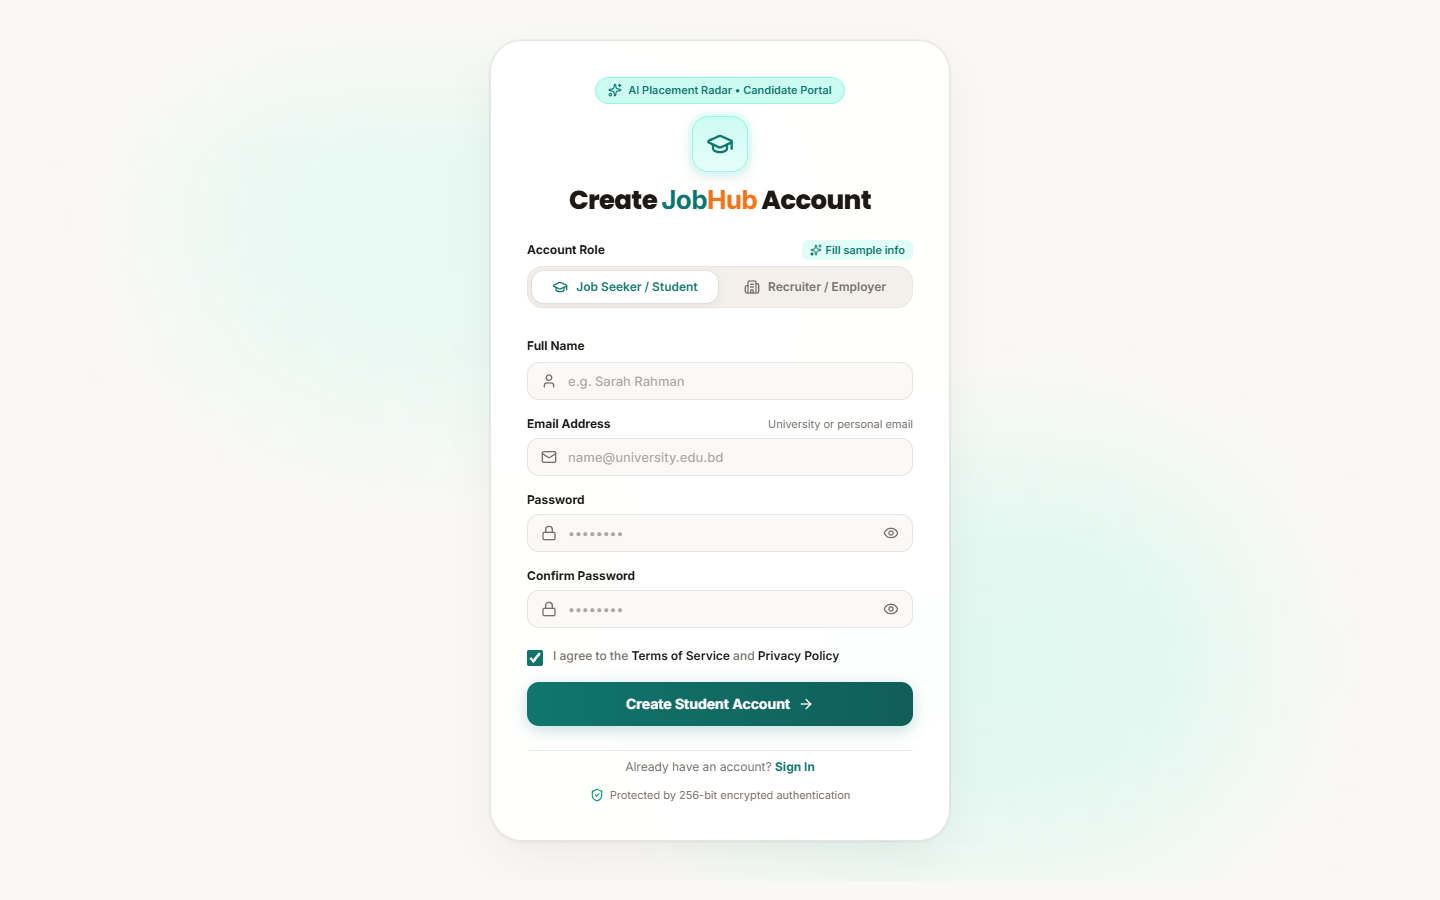
\includegraphics[width=0.92\textwidth]{assessment1_screenshots/01_register_seeker.png}
    \caption{\textbf{User Registration Page -- Job Seeker / Student View}\newline
    \textit{\small Displays the student registration form, dual-role selector tabs, and clean Nordic input styling.}}
    \label{fig:register_seeker}
\end{figure}

\vspace{1.5em}

\begin{figure}[H]
    \centering
    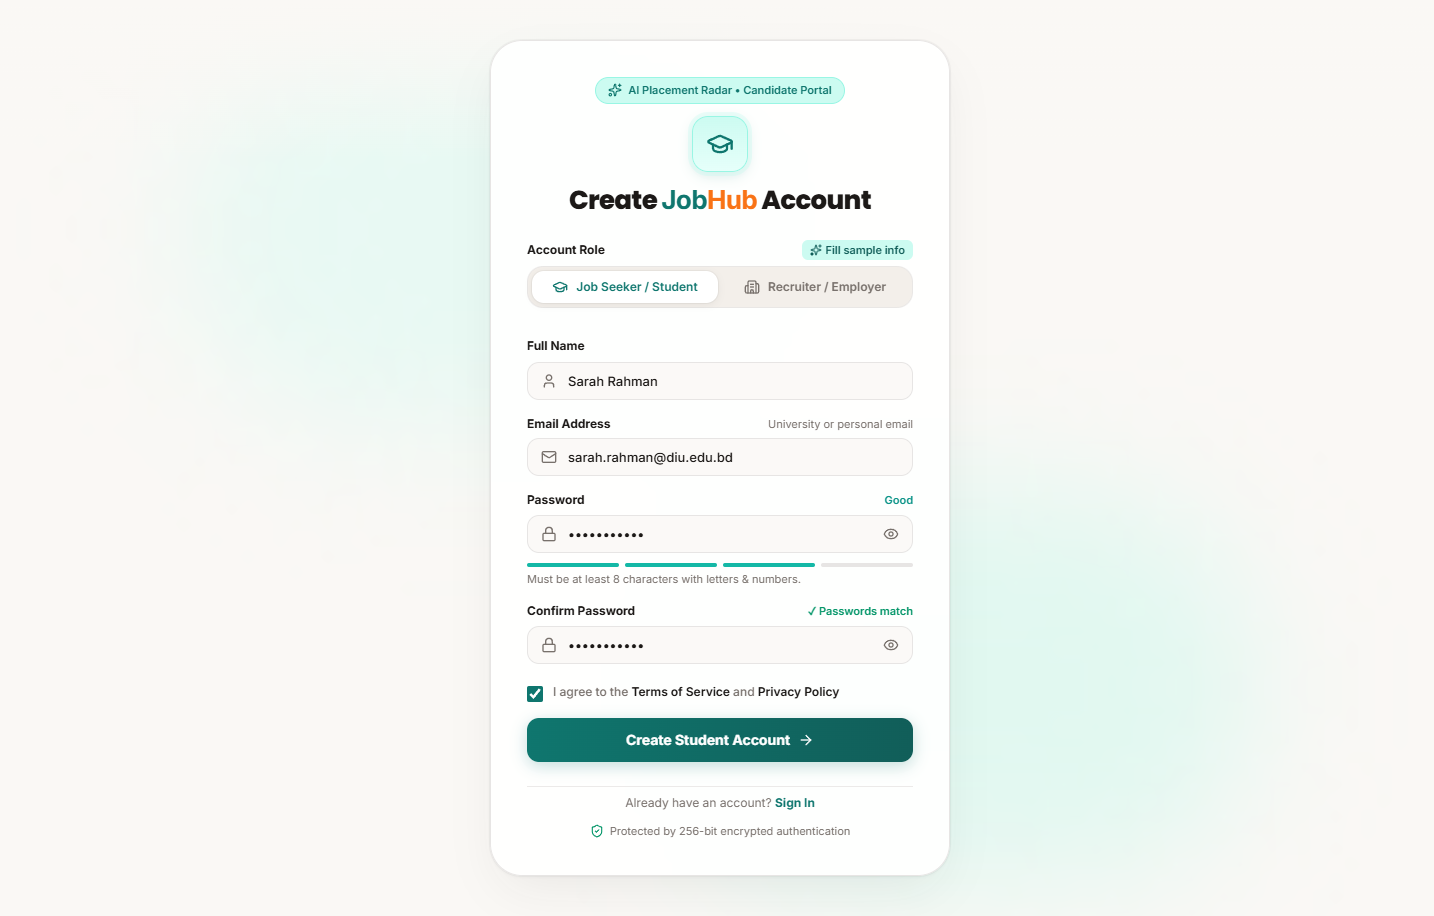
\includegraphics[width=0.92\textwidth]{assessment1_screenshots/02_register_seeker_filled_strength.png}
    \caption{\textbf{User Registration Page -- Dynamic Password Strength Meter}\newline
    \textit{\small Demonstrates real-time password entropy scoring (Good/Strong tier), visual progress indicator, and terms consent.}}
    \label{fig:register_strength}
\end{figure}

\newpage

\begin{figure}[H]
    \centering
    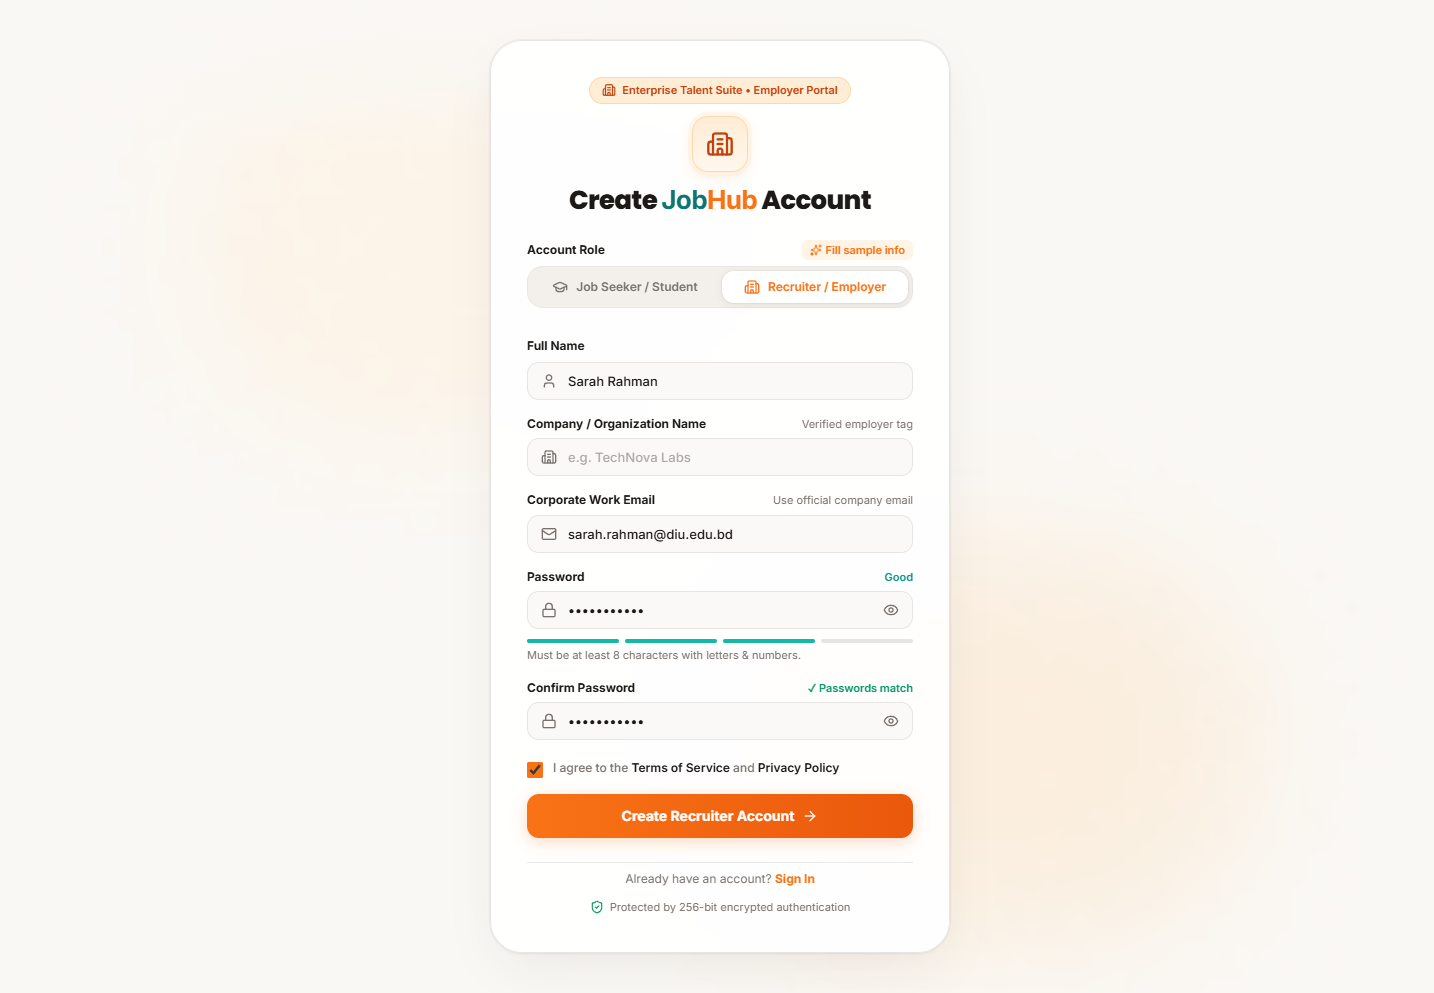
\includegraphics[width=0.92\textwidth]{assessment1_screenshots/03_register_recruiter.png}
    \caption{\textbf{User Registration Page -- Recruiter / Employer View}\newline
    \textit{\small Shows dynamic input adaptation: 'Full Name' switches to 'Company Name' and corporate work email format.}}
    \label{fig:register_recruiter}
\end{figure}

\vspace{1.5em}

\begin{figure}[H]
    \centering
    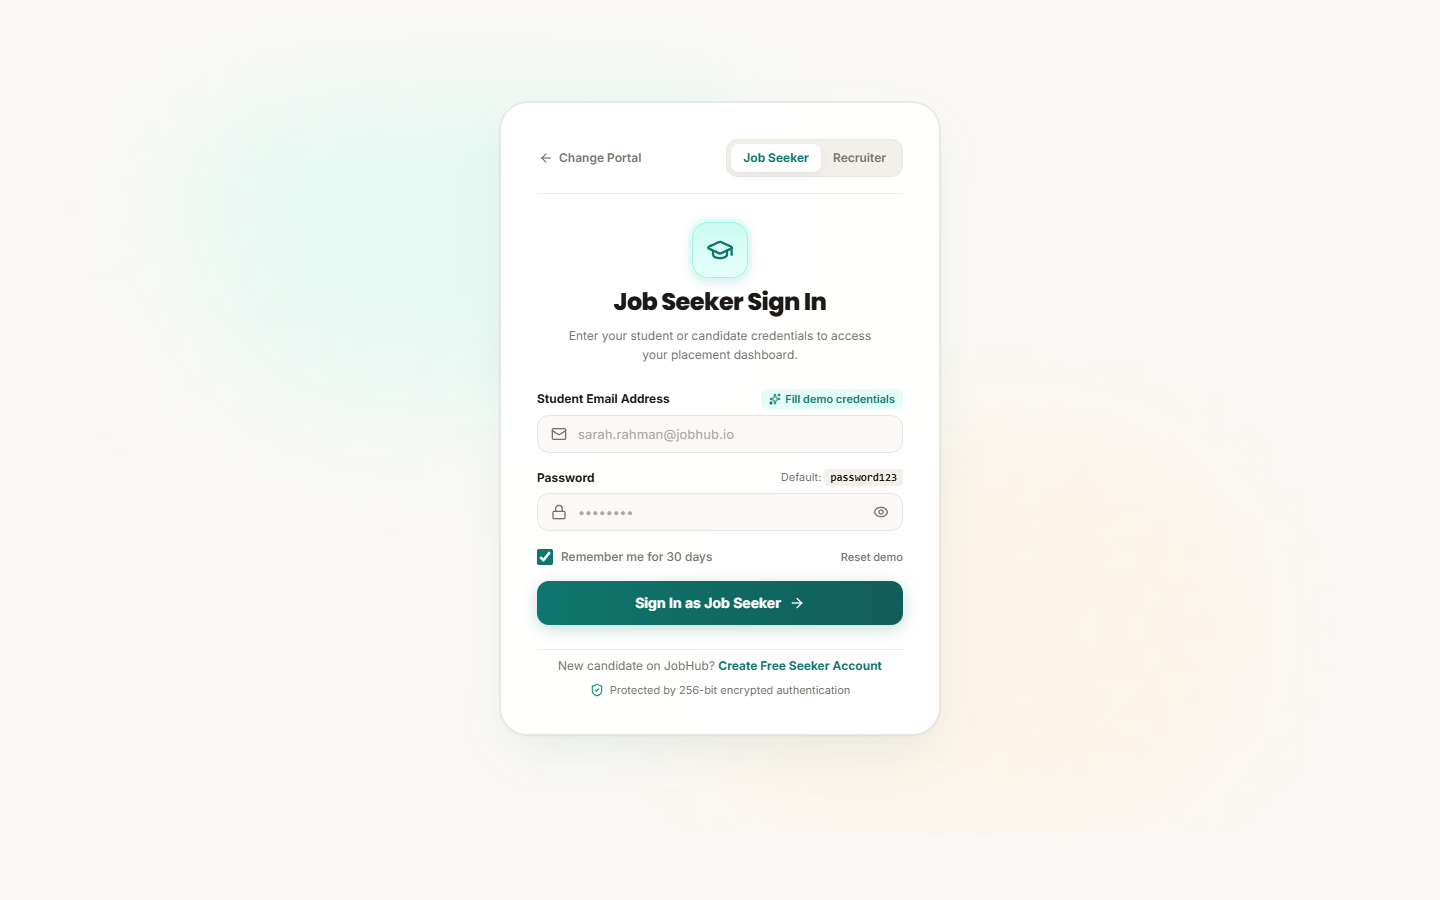
\includegraphics[width=0.92\textwidth]{assessment1_screenshots/04_login_page.png}
    \caption{\textbf{Sign In Authentication Gateway}\newline
    \textit{\small Role-based candidate and employer login portal with quick prefill assistance for evaluation.}}
    \label{fig:login_page}
\end{figure}

\newpage

\begin{figure}[H]
    \centering
    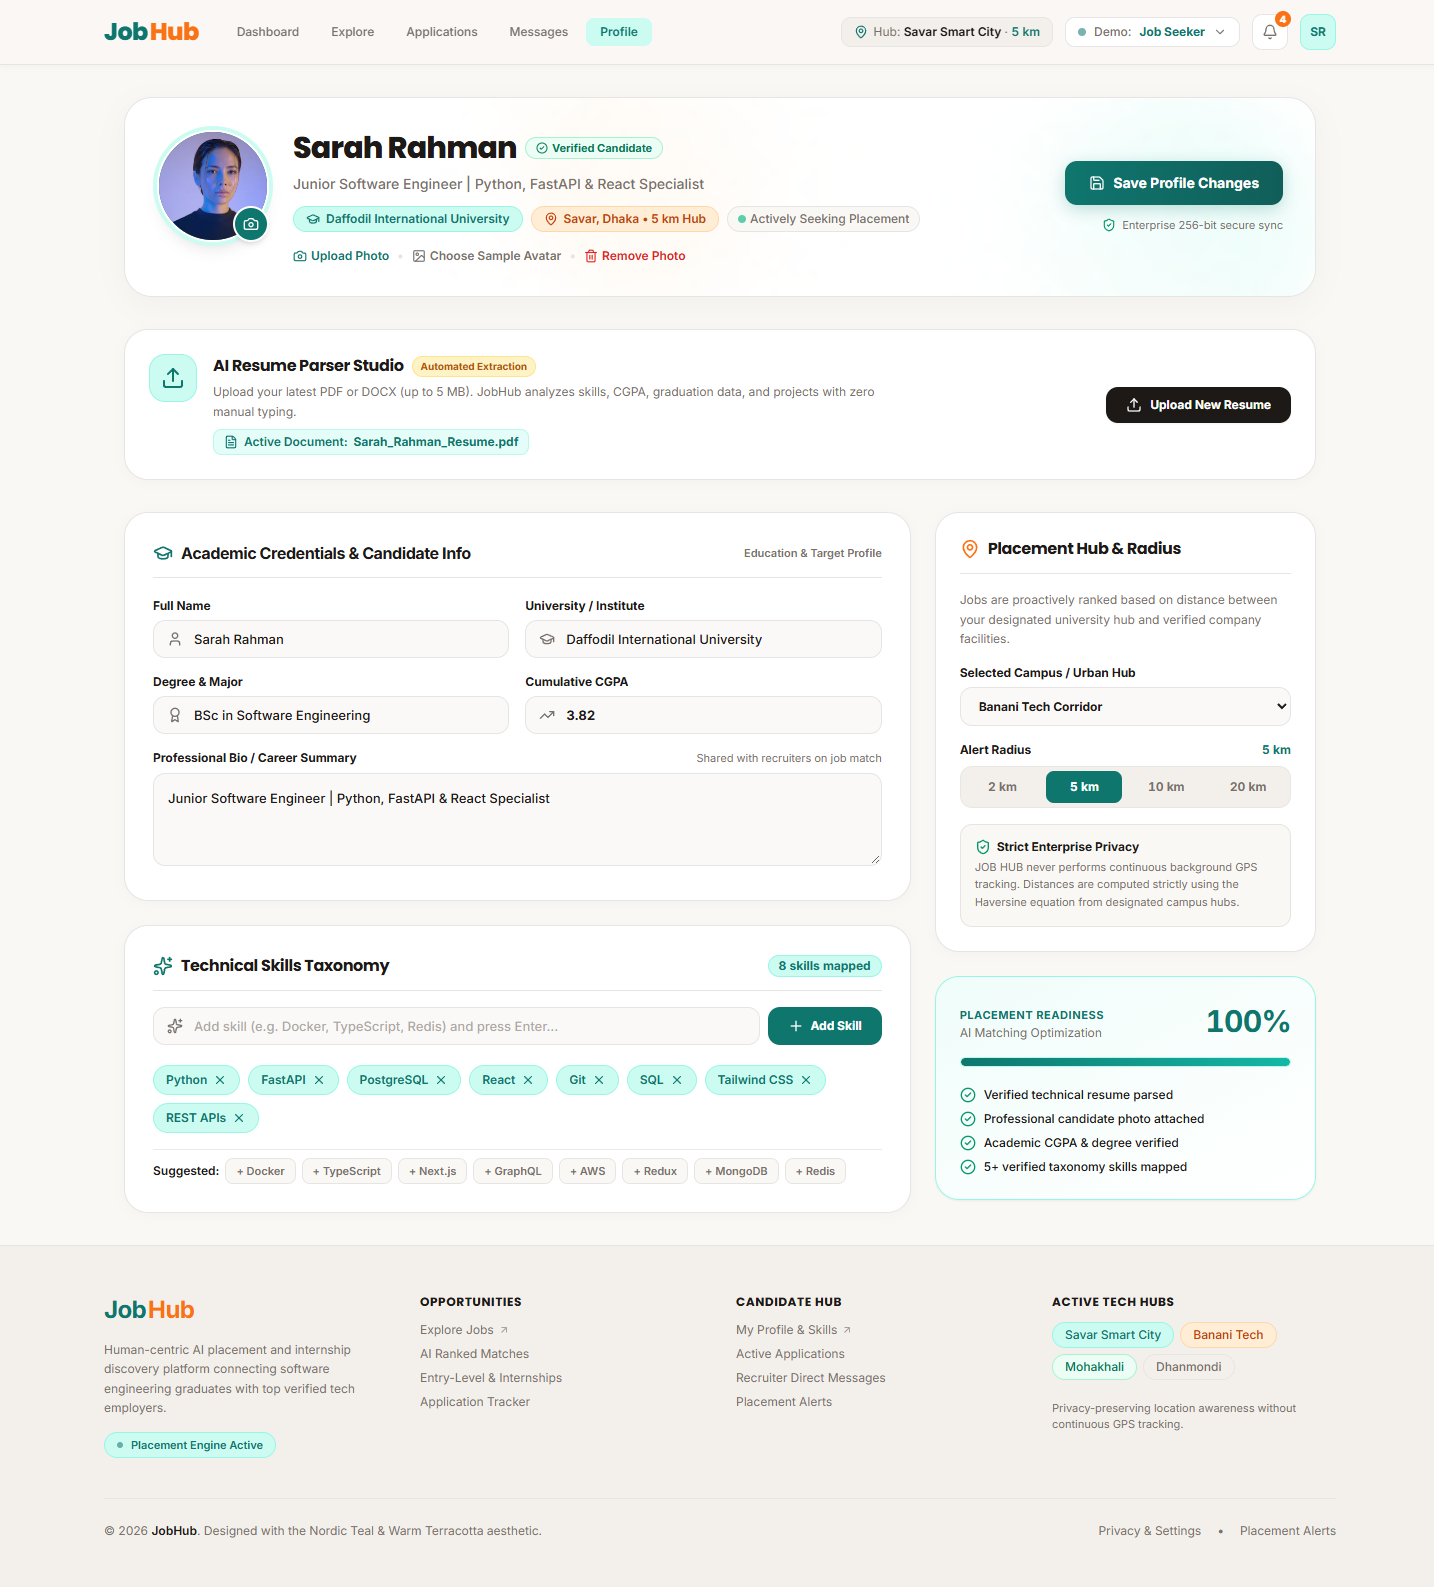
\includegraphics[width=0.88\textwidth]{assessment1_screenshots/05_seeker_profile_full.png}
    \caption{\textbf{Candidate Profile Management Screen (\texttt{/profile})}\newline
    \textit{\small Complete view of the Job Seeker profile featuring AI Resume Studio, Academic Credentials (DIU, BSc SWE, CGPA 3.82), Skills Taxonomy, and Geospatial Placement Radar.}}
    \label{fig:profile_full}
\end{figure}

\newpage

\begin{figure}[H]
    \centering
    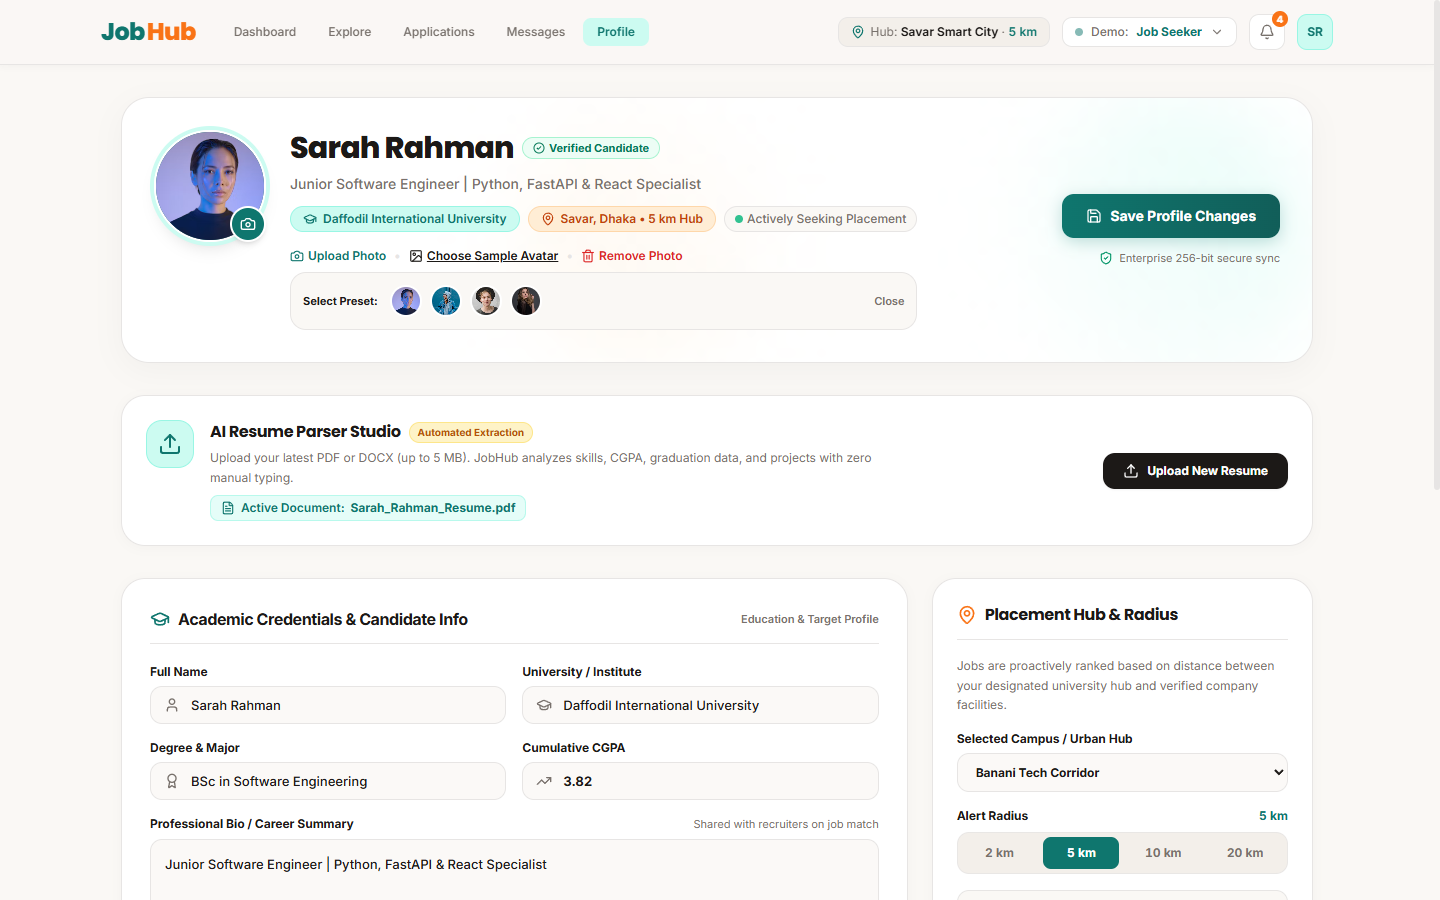
\includegraphics[width=0.92\textwidth]{assessment1_screenshots/06_avatar_modal.png}
    \caption{\textbf{Interactive Avatar Chooser Modal}\newline
    \textit{\small Modal dialog offering curated professional avatar presets with client-side image compression and photo preview.}}
    \label{fig:avatar_modal}
\end{figure}

\vspace{1.5em}

\begin{figure}[H]
    \centering
    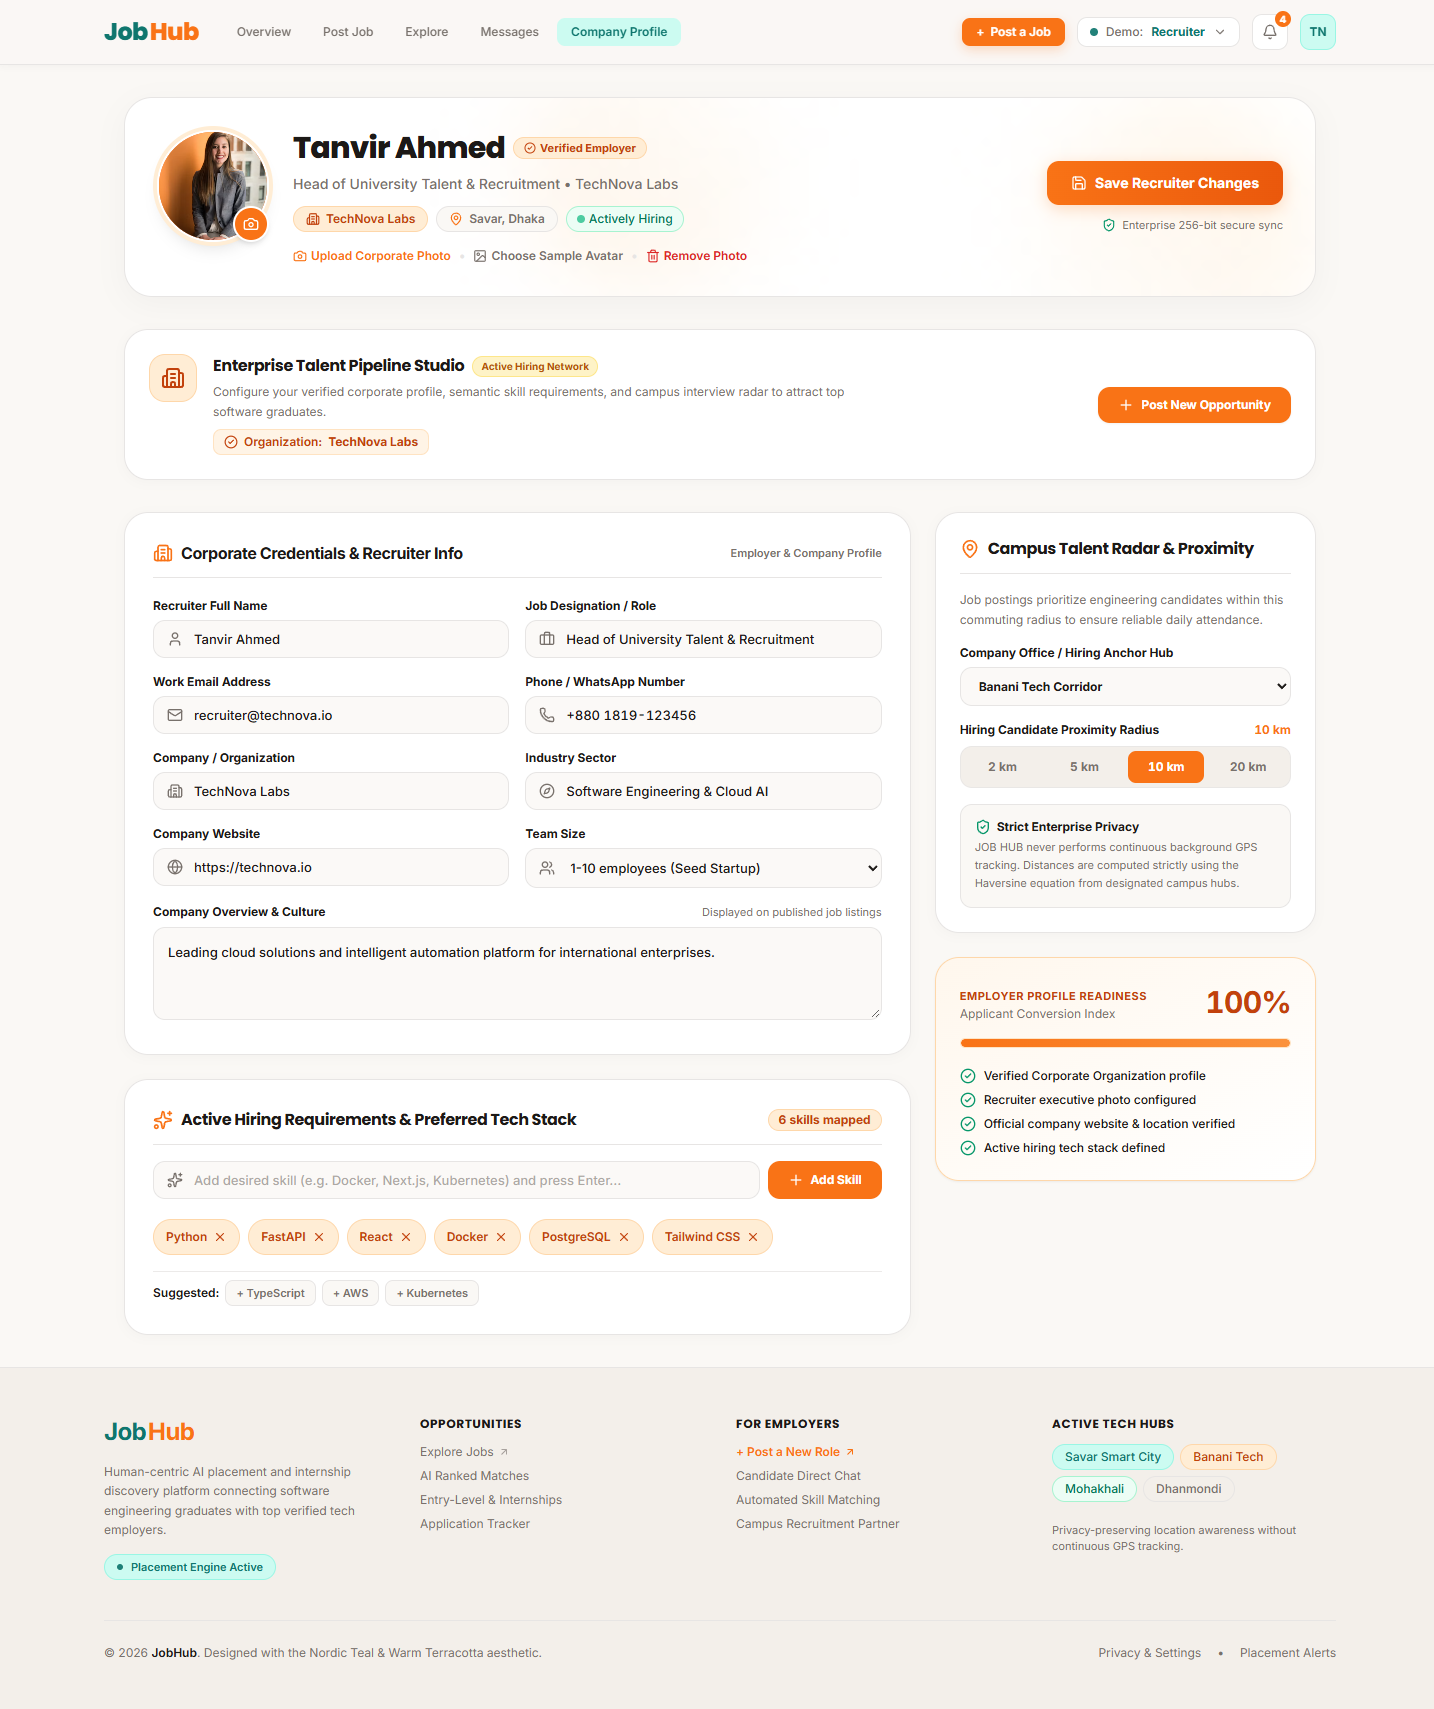
\includegraphics[width=0.88\textwidth]{assessment1_screenshots/07_recruiter_profile_full.png}
    \caption{\textbf{Recruiter Corporate Profile Screen (\texttt{/profile})}\newline
    \textit{\small Recruiter organization view featuring company size, industry classification, corporate website, Banani office anchor, and hiring tech stack.}}
    \label{fig:recruiter_profile}
\end{figure}

\newpage

\begin{figure}[H]
    \centering
    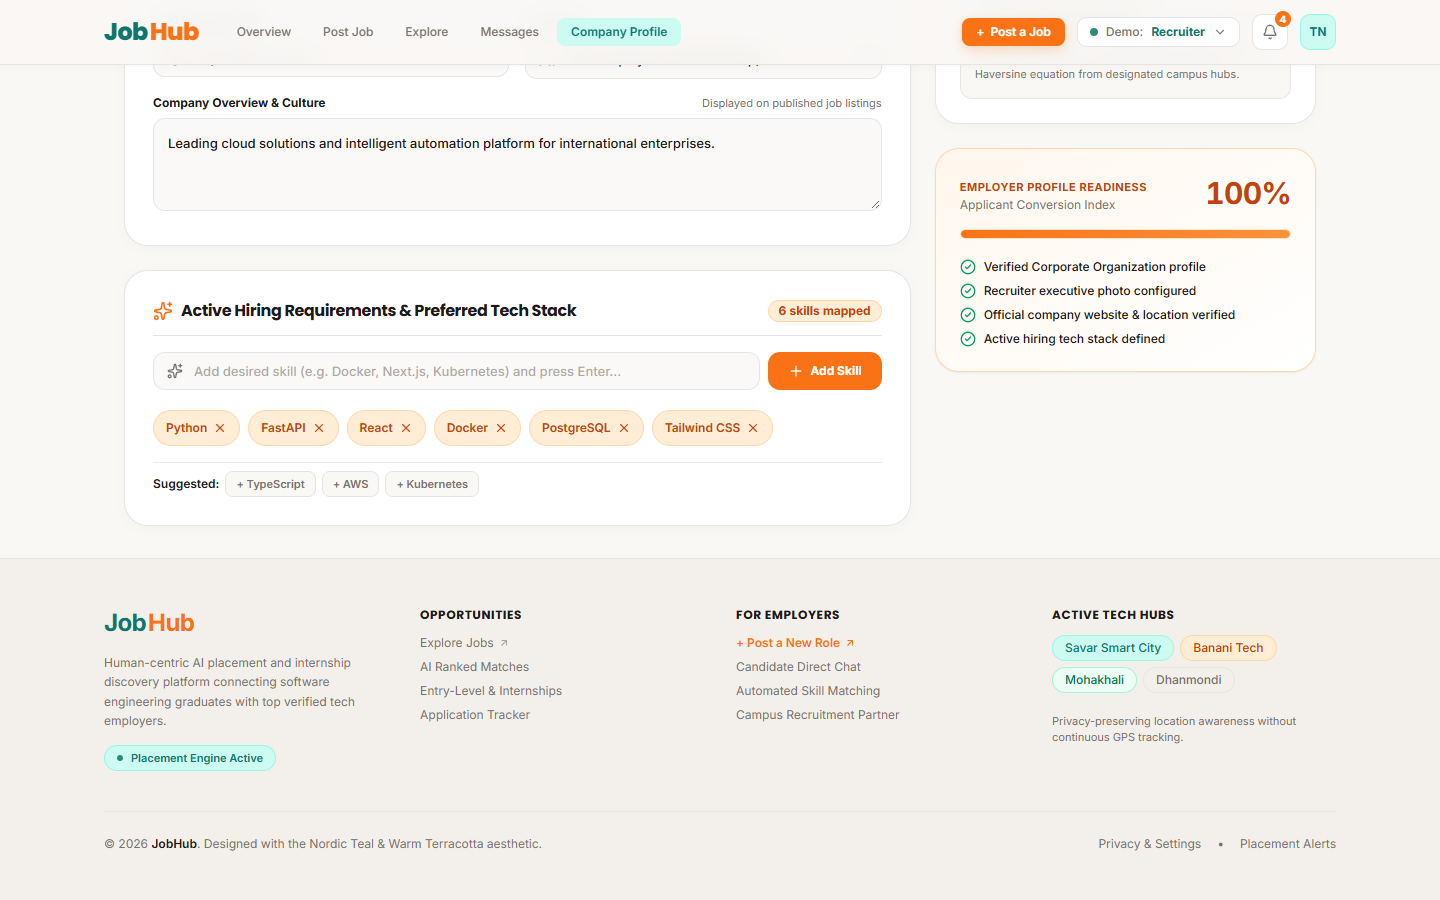
\includegraphics[width=0.92\textwidth]{assessment1_screenshots/08_interactive_skills_chips.png}
    \caption{\textbf{Interactive Skills Taxonomy Management}\newline
    \textit{\small Demonstrates dynamic chip additions (\texttt{+ TypeScript}, \texttt{+ AWS}), tag removal buttons, and live taxonomy count indicator.}}
    \label{fig:skills_chips}
\end{figure}

\vspace{1.5em}

% -----------------------------------------------------------------------------
% 6. Verification & Prototype Access Links
% -----------------------------------------------------------------------------
\section{Verification \& Prototype Access Links}

The interactive prototype is fully operational and can be reviewed via the following channels:

\begin{itemize}[leftmargin=1.5em, itemsep=0.4em]
    \item \textbf{Live Cloud Prototype (GitHub Pages):} \url{https://saif-alsaad.github.io/JobHub/}\newline
    \textit{\small Directly accessible via any web browser, zero local dependencies or configuration required.}
    \item \textbf{Official Repository Sub-Branch:} \url{https://github.com/Saif-AlSaad/JobHub/tree/Nadim}
    \item \textbf{Evaluation Test Credentials:}
    \begin{itemize}[leftmargin=1.2em, itemsep=0.2em]
        \item \textbf{Job Seeker:} \texttt{sarah.rahman@jobhub.io} / \texttt{password123}
        \item \textbf{Recruiter:} \texttt{recruiter@technova.io} / \texttt{password123}
        \item \textbf{Administrator:} \texttt{admin@jobhub.io} / \texttt{password123}
    \end{itemize}
\end{itemize}

\end{document}

